\documentclass[a4paper,12pt]{article}
\usepackage[utf8]{inputenc}
\usepackage{graphicx}
\usepackage{indentfirst}
\graphicspath{ {img/} }

\setlength{\oddsidemargin}{0mm}
\setlength{\evensidemargin}{-14mm}
\setlength{\marginparwidth}{0cm}
\setlength{\marginparsep}{0cm}
\setlength{\topmargin}{2mm}
\setlength{\headheight}{0mm}
\setlength{\headsep}{0cm}
\setlength{\textheight}{240mm}
\setlength{\textwidth}{168mm}
\setlength{\topskip}{0mm}
\setlength{\footskip}{10mm}
\setlength{\parindent}{8ex}

\begin{document}
	\begin{titlepage}
    	\begin{center}
        	\vspace*{1cm}
        
        	\textbf{Mobile Data Collection in Wireless Delay Tolerant Networks}
        
        	\vspace{0.5cm}
        	Progress Report
        
        	\vspace{1.5cm}
        
        	\textbf{Jono Kapene \\ 53044694}
        
        	\vfill
        	
\includegraphics[scale=0.8]{Tait-Communications-logo.png}\\
        		
        	\vspace{0.8cm}
        
        	Group E16\\
        	University of Canterbury\\
        	15th May, 2017
        
		\end{center}
	\end{titlepage}

	\clearpage
	\tableofcontents
	\listoffigures
	\listoftables
	\clearpage
	
	
\section{Abstract}
\clearpage

\section{Project Overview}
Tait communications is a Christchurch based telecommunications service provider and the sponsor of this project. Tait has over 47 years experience in radio and critical communications which makes there target market primarily emergency services utility operators who have a need for reliability and ease of implementation. One of Taits' core values is "integrity to deliver what they promise". This is important to the group as its these values that we need to deliver in order for tait to be satisfied.\\

Tait have set us the goal to create a sensor network that communicates to a vehicle area network (VAN) for data collection and the whole system must be delay tolerant. The specific application for such a product was for the group to research and decide. Other components Tait wanted the solution to include were a cloud storage system, a back office application and some way to graphically display the data being harvested to a driver in the VAN. Before any design work started, Tait wanted the group to survey the possible technologies to use in our delay tolerant network. There are a number of technologies that seemed plausible and a review of each was needed to be done. After researching and designing was complete we were to create a "proof of concept" prototype using their existing platform Unify Vehicle.\\

Unify Vehicle was developed to aid in one of their other products, Unify Voice. Unify Voice is a system that allows the user to communicate over multiple networks depending on their environmental circumstances to give them the best possible coverage. The Unify Vehicle was used in this system as a gateway to these networks in the form of an on-board unit for the users vehicle. Unify Vehicle, for this project, can be described as a Linux based embedded system which can communicate over Wi-Fi, Bluetooth and digital mobile radio (DMR). Tait have given the group a UV unit, however they have disabled radio transmission so we don't break any broadcasting laws. This has limited the scope of the project to not be able to use DMR. \\


\clearpage

\section{Progress To Date}

At the start of the project we were to choose an application for our prototype. The group, as a whole, started to brainstorm and research possible applications and the best ideas were listed below:

\begin{enumerate}
\item Sensor data collection for farmers.
\item asset tracking inside mines.
\item Portable network for search and rescue.
\end{enumerate}

In the end Tait had suggested the asset tracking for mines and set up a meeting  for us with one of their mining consultants, Bruce Magee. Bruce has experience working in mines all around the world and shared some of his knowledge with us. The main points we got from his meeting were that there was a need for the system we described. That system was the asset tracker.\\

In open cast mines a big problem they had was that equipment was often lost. Bruce told us about how lamps and water pumps were misplaced or blown up daily. Most of the time people just forgot where they had last put something and then spend sometimes hours driving around the mine looking for it. All of this stuff was inexpensive in comparison to the other mining equipment but cost them a lot of time when they couldn't find them. There was also strict maintenance schedules on all of this equipment and the maintenance team had no way of tracking where these item were when it came time to check them.\\

The miners Bruce had worked for also didn't like spending lots of time implementing a system and then have to maintain it. Often they would implement a system and after a while it would start to not work they would just throw the system out. So once a system was implemented the little maintenance required the better.\\

\clearpage
\begin{flushleft}
\subsection{Research}
\end{flushleft}

I am in charge of programming the UV and the first step was to do some research. The main information i wanted to find out first was whether there was already an existing solution. A similar delay tolerant system was prototyped by Universidade de Aveiro. It used a bus to transport sensor information back to a relay point. Data collection units (DCU), made up of sensors, Wi-Fi module and a raspberry pi, were placed on roadside lamp post around the city to collect weather information. The data was stored in the DCU until it was transmitted to an on board unit (OBU)in a passing bus via Wi-Fi. The bus would then pass a road side unit (RSU)where the data will be again transmitted by Wi-Fi and then sent to a back end server via fibre connection. This system has two delay tolerant connections. One between the DCU and  the OBU, and another between the OBU and the RSU. The buses were all  part  of the same network, allowing data to be transmitted from bus to bus. Figure \ref{figure:exs1}

\begin{figure}[h!]
\begin{center}
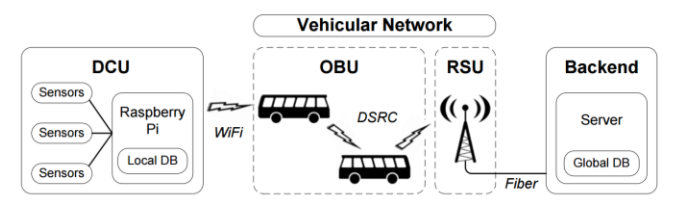
\includegraphics[scale=0.46]{/exs.png}
\caption{Physical architecture of the collection platform}
\label{figure:exs1}
\end{center}
\end{figure}

Another useful project we could get ideas from was a beagle bone GPS tracker. The Beagle Bone is software compatible with Unify Vehicle. A hobbyist youtuber has created a GPS tracker using a beagle bone and a GPS breakout board. The information gets uploaded to his home computer and displays it on google earth. The beagle bone mimics our Unify vehicle and we can adapt the way the information gets to it form the GPS breakout board. Displaying the information on google earth might suit our project considering we need a back-office display.\\

\subsection{Building Prototype}

The group decided to build a simple prototype to start with. The prototype was going to simply send 1 bit of data from the Lora terminal all the way through to a back end display. I was tasked with 

\clearpage
\section{Remaining Tasks}
The next immediate steps that need to take place is firstly to demonstrate the system prototype to Bruce. We need to get feedback on what key features he thinks the system should have and what priority those features have. The project currently has no way of displaying sensor data to someone inside the VAN. We have already decided on using a web app that can be hosted by a back end server and then cached by the UV when its out of internet range. This will allow any device that can read a web-page, such as a mobile phone or a laptop, to have access to that data.\\

Work on the web app will need to start after the stakeholder meeting with Bruce. That meeting will be a good time to get an idea of what functionalities the web app will need to have. Currently the system is not delay tolerant. This is a key feature our system needs to have and will most likely take the longest to implement. Every group member will be needed to implement this as it affects everyone sections. The LoRa sensor terminal needs to have a sensor added so we can start testing the system with actual data.\\

\begin{flushleft}
Major tasks that I will need to complete in the immediate future:
\end{flushleft}
\begin{enumerate}
\item Write a python program for the UV to cache and display the web app.
\item Edit connections from base station to UV and UV to back end server so they are delay tolerant. 
\end{enumerate}
\begin{figure}[h!]
\begin{center}
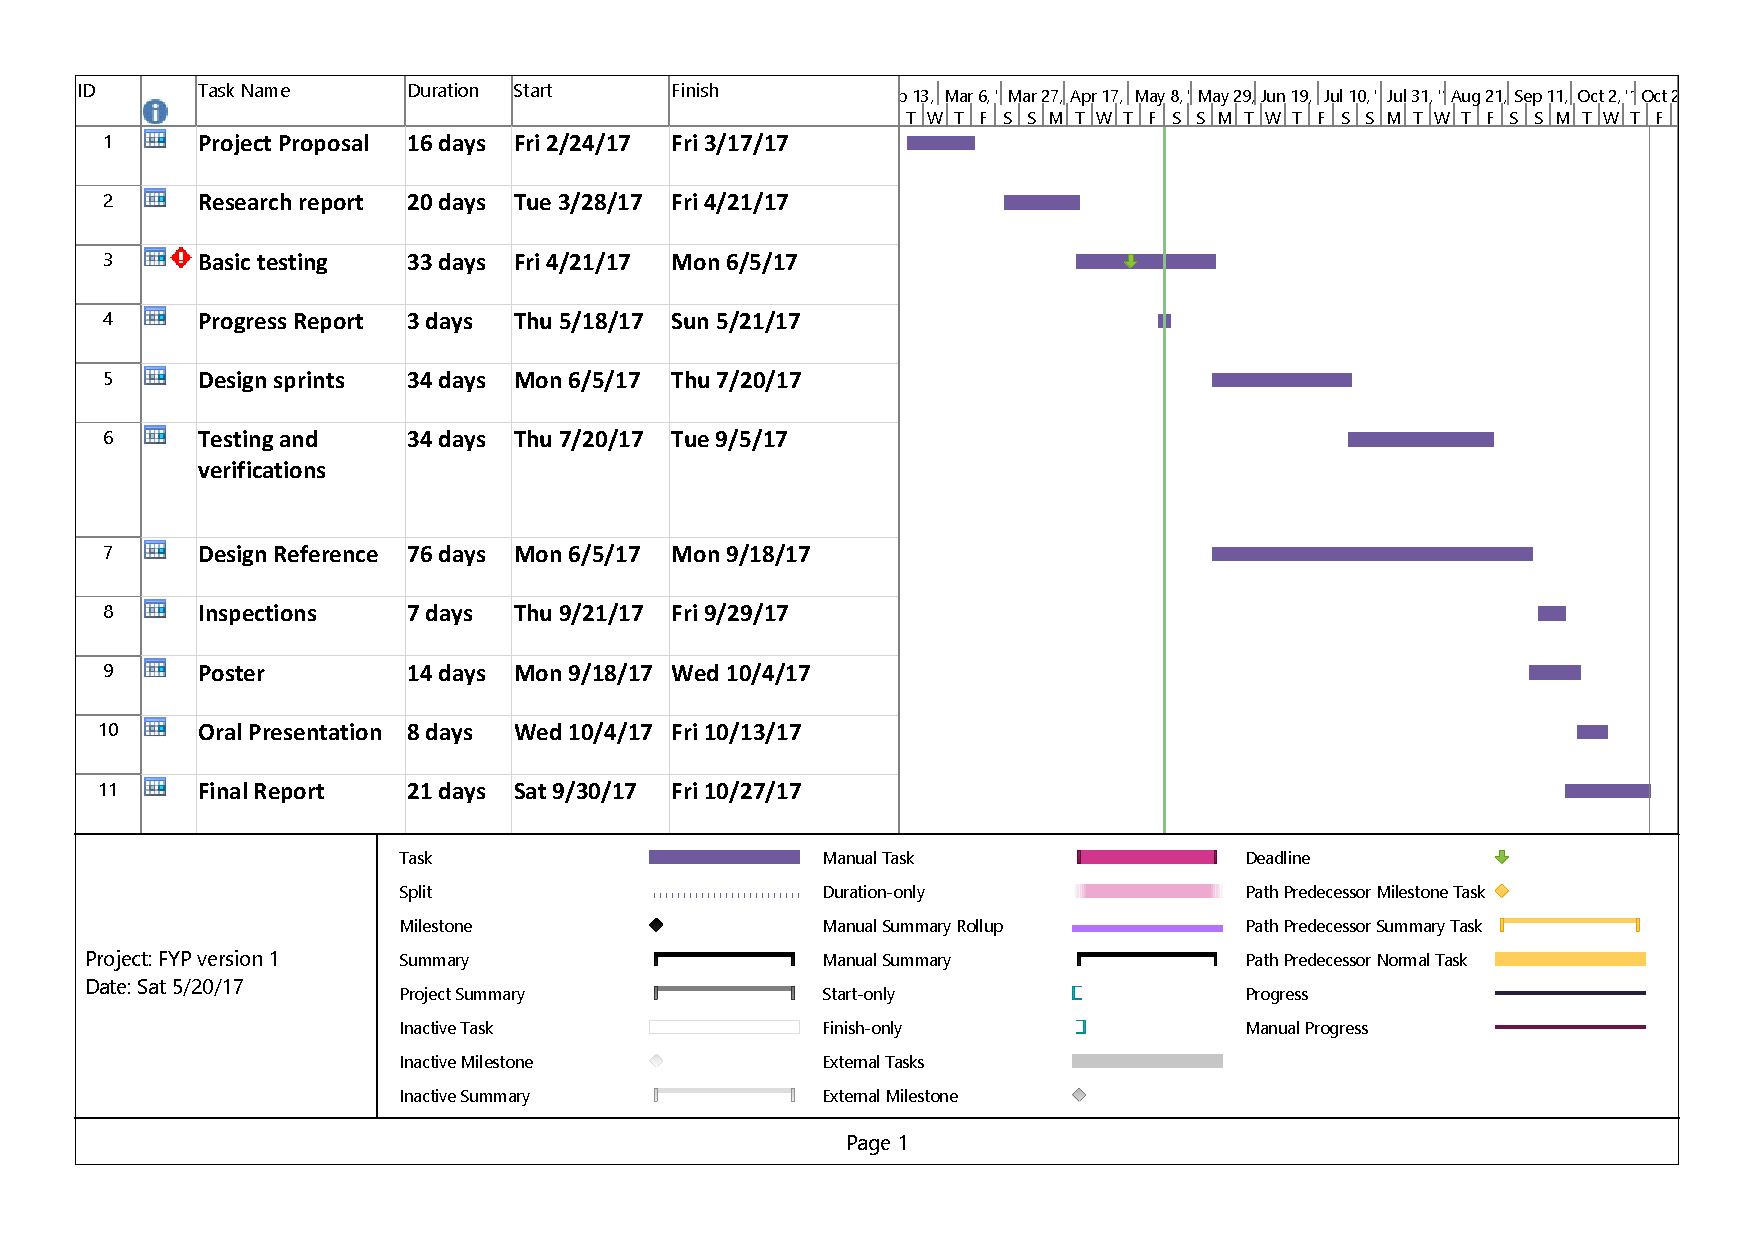
\includegraphics[scale=0.46]{gnattchart2.pdf}
\caption{Updated gantt chart for the overall project.}
\label{figure:gantt}
\end{center}
\end{figure}

\clearpage
\section{Sustainability Analysis}
\clearpage
\section{Budget Summary}

\begin{table}[h!]
\begin{center}
\caption{Price of items purchased as of 20/05/2017}
\begin{tabular}{||c|c|c|c||} 
 \hline
 Item & Qty & Price\\
 \hline
 \hline
 Pycom LoPy development board & 2 & \$96.62 \\
 \hline
 Pycom universal antenna kit & 2 & 40.00\\
 \hline 
 Pycom Universal Expansion board 2.0 & 1 & \$37.50 \\ 
 \hline
  & Total &  174.12\\ 
 \hline
\end{tabular}
\label{table:purchases}
\end{center}
\end{table}

The group has a budget of \$250 for this project however the WRC have said they are willing to cover expenses if we go a little over budget. Table \ref{table:purchases} shows the items the group has felt necessary to purchase for our project. We have received all items in this table and have ordered nothing more. \\

\begin{figure}[h!]
\begin{center}
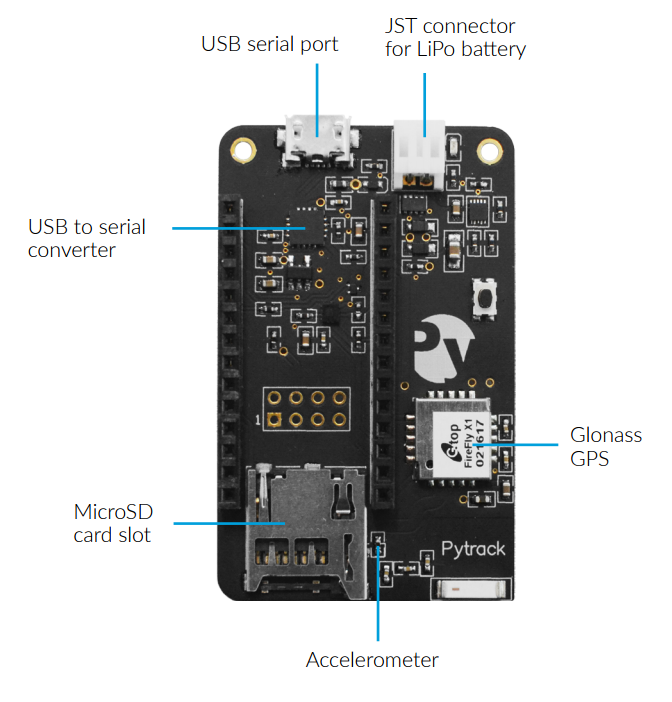
\includegraphics[scale=0.3]{pytrack.png}
\caption{Pytrack modules key features}
\label{figure:pytrack}
\end{center}
\end{figure}

That leaves us with ~\$75 left. We are interested in placing an order for a GPS module, Pytrack, shown in figure \ref{figure:pytrack}. This would integrate into the system we have now very easily as its made by the same people as all our other purchases and would work out of the box. This particular module has only been released recently which is why we have not yet placed an order for it. The estimated price for the Pytrack is \$65 including shipping, however this is subject to the euro exchange rate.\\

We do already have a GPS module from last years project but its not the best quality and would take time to set up. The Pytrack purchase would use almost all of the remaining budget so we are delaying the purchase in-case we need that money for something more important. As of 18th of May, we are not looking for any other purchases.

\clearpage

\section{Conclusions}
\clearpage
\section{References}

\end{document}